\documentclass[a4paper, landscape]{article}

\usepackage[utf8]{inputenc}
\usepackage[DIV=12]{typearea}
\usepackage{microtype}
\usepackage{float}
\usepackage{mathtools, amssymb}
\usepackage{parskip}
\usepackage{subcaption}
\usepackage{graphicx}
\usepackage[colorlinks=true]{hyperref}

\title{9}
\date{} 

\graphicspath{ {../images} }

\hypersetup{linktoc=all}

\setlength{\parindent}{0em}

\begin{document}
\maketitle

\section{Images}
\ref{lc1_orig} and \ref{lc2_orig} are the original images. The block size used for Adaptive Histogram Equalization increases as you go to the right and downwards, with the first image in both series being the original image and the last image (again, in both series) having been enhanced using Global Histogram Equalization.


\begin{figure}
    \centering
    \begin{subfigure}{0.32\linewidth}
        \centering
        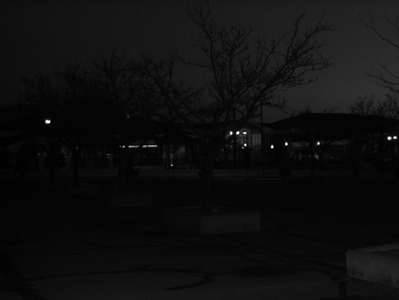
\includegraphics[width=\linewidth]{LC1.png}
        \caption{Given image, without any enhancements of any kind.}
        \label{lc1_orig}
    \end{subfigure}
    \begin{subfigure}{0.32\linewidth}
        \centering
        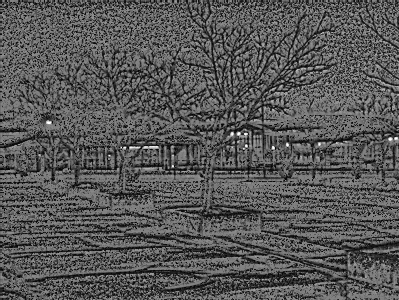
\includegraphics[width=\linewidth, keepaspectratio]{smol_enhanced_LC1.png}
        \caption{Image enhanced using Adaptive Histogram Equalization with $7\times 7$ blocks.}
    \end{subfigure}
    \begin{subfigure}{0.32\linewidth}
        \centering
        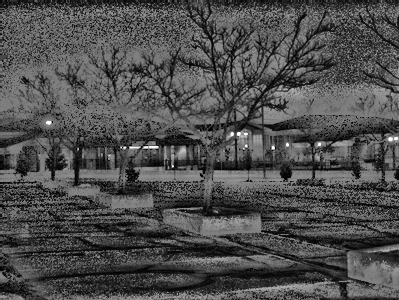
\includegraphics[width=\linewidth]{medium_enhanced_LC1.png}
        \caption{Image enhanced using Adaptive Histogram Equalization with $31\times 31$ blocks.}
    \end{subfigure}
\end{figure}
\begin{figure}
    \centering
    \begin{subfigure}{0.32\linewidth}
        \centering
        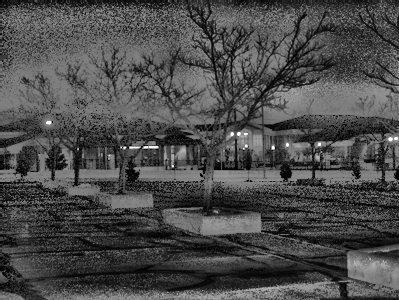
\includegraphics[width=\linewidth]{big_enhanced_LC1.png}
        \caption{Image enhanced using Adaptive Histogram Equalization with $51\times 51$ blocks.}
    \end{subfigure}
    \begin{subfigure}{0.32\linewidth}
        \centering
        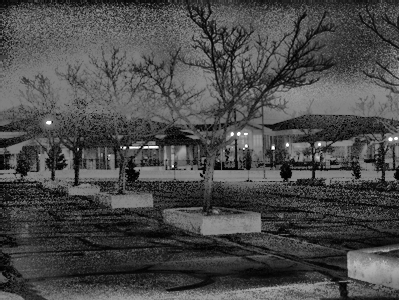
\includegraphics[width=\linewidth]{chonky_enhanced_LC1.png}
        \caption{Image enhanced using Adaptive Histogram Equalization with $71\times 71$ blocks.}
    \end{subfigure}
    \begin{subfigure}{0.32\linewidth}
        \centering
        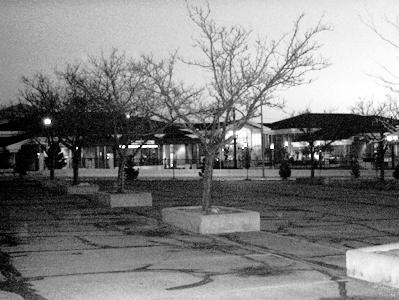
\includegraphics[width=\linewidth]{global_histogram_LC1.jpg}
        \caption{Image enhanced using Global Histogram Equalization.}
    \end{subfigure}
\end{figure}

\begin{figure}
    \centering
    \begin{subfigure}{0.32\linewidth}
        \centering
        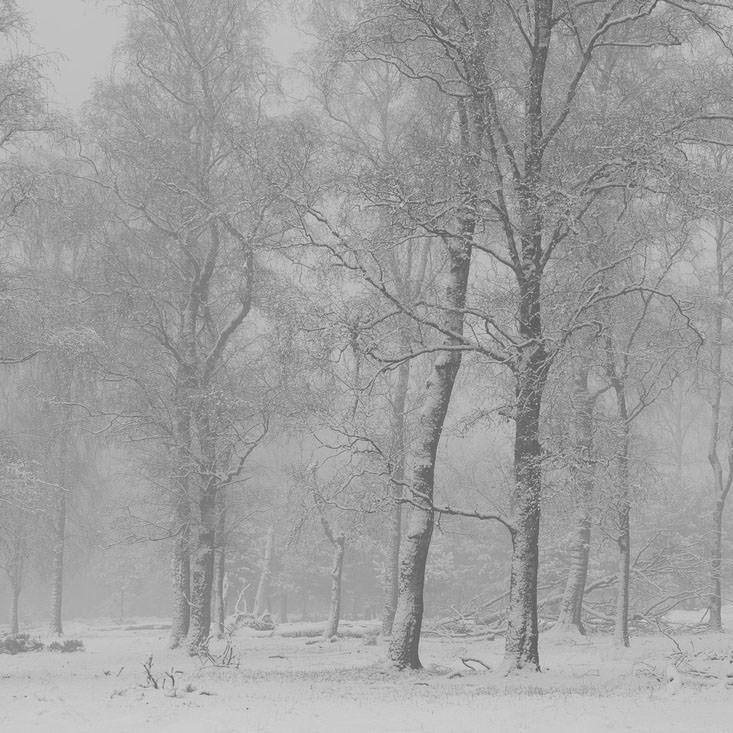
\includegraphics[height=0.4\textheight, keepaspectratio]{LC2.jpg}
        \caption{Given image, without any enhancements of any kind.}
        \label{lc2_orig}
    \end{subfigure}
    \begin{subfigure}{0.32\linewidth}
        \centering
        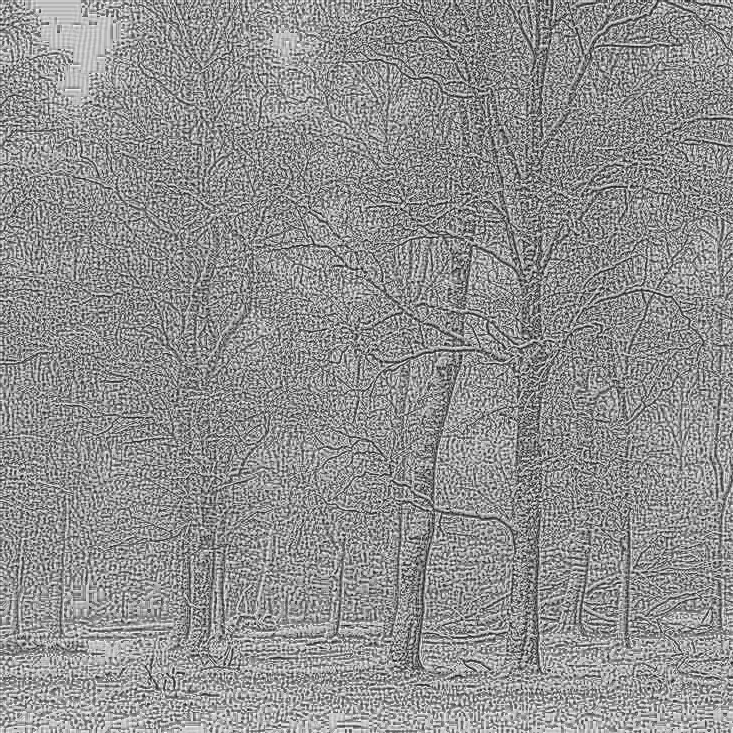
\includegraphics[height=0.4\textheight, keepaspectratio]{smol_enhanced_LC2.png}
        \caption{Image enhanced using Adaptive Histogram Equalization with $7\times 7$ blocks.}
    \end{subfigure}
    \begin{subfigure}{0.32\linewidth}
        \centering
        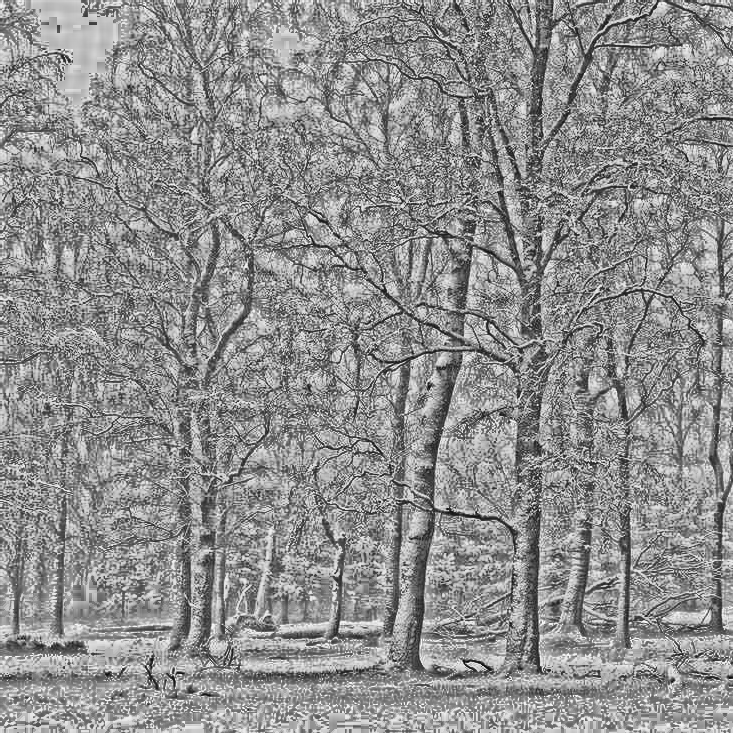
\includegraphics[height=0.4\textheight, keepaspectratio]{medium_enhanced_LC2.png}
        \caption{Image enhanced using Adaptive Histogram Equalization with $31\times 31$ blocks.}
    \end{subfigure}
\end{figure}
\begin{figure}
    \centering
    \begin{subfigure}{0.32\linewidth}
        \centering
        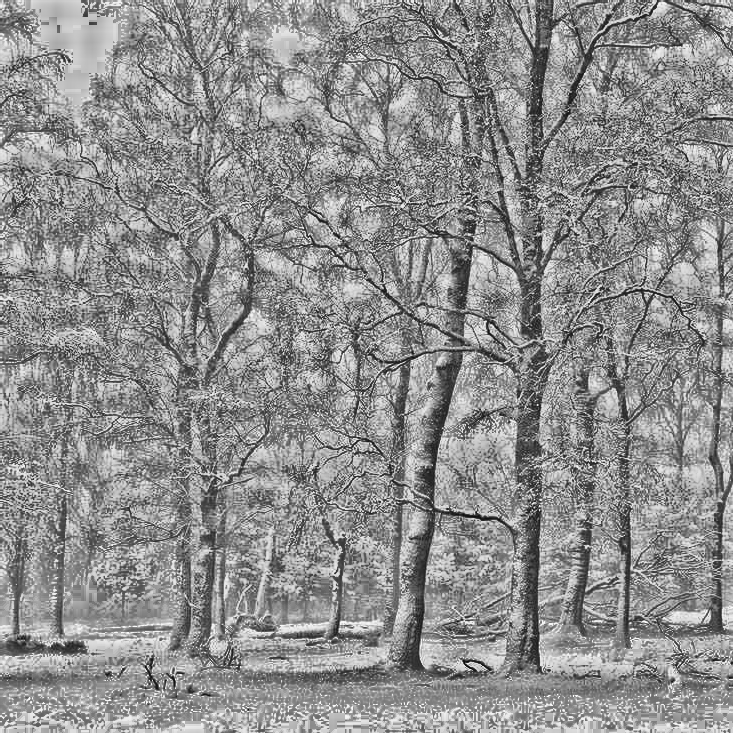
\includegraphics[height=0.4\textheight, keepaspectratio]{big_enhanced_LC2.png}
        \caption{Image enhanced using Adaptive Histogram Equalization with $51\times 51$ blocks.}
    \end{subfigure}
    \begin{subfigure}{0.32\linewidth}
        \centering
        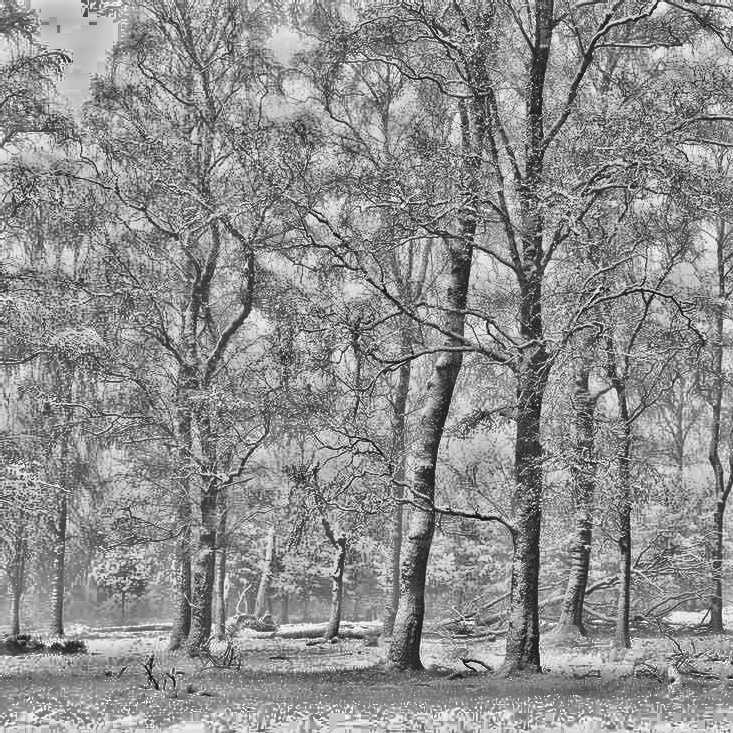
\includegraphics[height=0.4\textheight, keepaspectratio]{chonky_enhanced_LC2.png}
        \caption{Image enhanced using Adaptive Histogram Equalization with $71\times 71$ blocks.}
    \end{subfigure}
    \begin{subfigure}{0.32\linewidth}
        \centering
        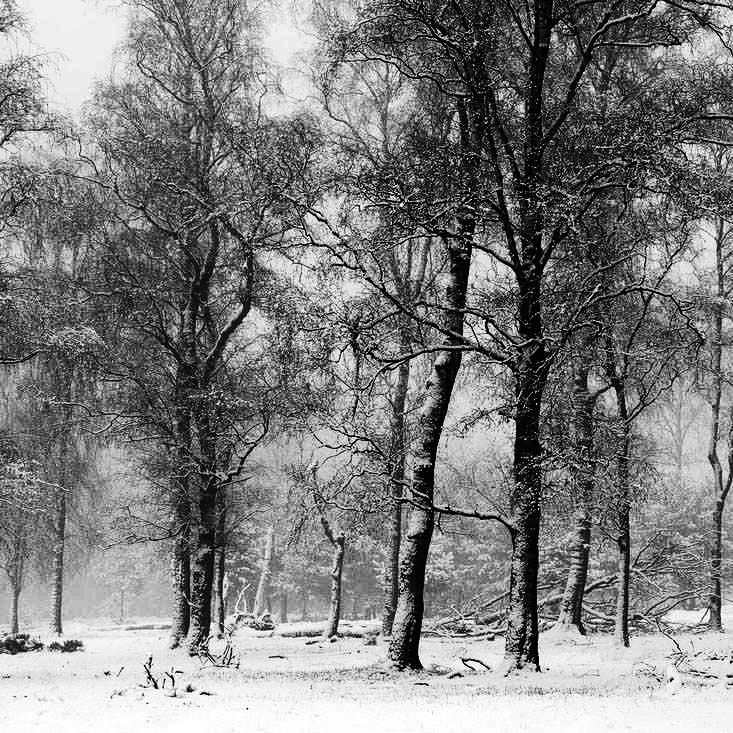
\includegraphics[height=0.4\textheight, keepaspectratio]{global_histogram_LC2.jpg}
		\caption{Image enhanced using Global Histogram Equalization.}
    \end{subfigure}
\end{figure}
\end{document}